\documentclass[12pt]{article}

\usepackage[a4paper,margin=0.75in]{geometry}
\usepackage{graphicx}
\usepackage{hyperref}
\usepackage{titlesec}
\usepackage{float}
\usepackage{booktabs}
\usepackage{array}
\usepackage{enumitem}
\usepackage{setspace}
\usepackage{parskip}
\usepackage{amsmath}
\usepackage{xcolor}
\usepackage{listings}
\usepackage{tabularx}
\usepackage{tcolorbox}
\usepackage{pdflscape}

% ---------------- Graphics Path ----------------
\graphicspath{{image/}{images_preksha_r1_r5/}{./}}

% ---------------- Formatting ----------------
\titleformat{\section}{\large\bfseries}{\thesection}{1em}{}
\titleformat{\subsection}{\normalsize\bfseries}{\thesubsection}{1em}{}
\titleformat{\subsubsection}{\small\bfseries}{\thesubsubsection}{1em}{}

\titlespacing*{\section}{0pt}{2.2ex}{1.2ex}
\titlespacing*{\subsection}{0pt}{1.8ex}{0.9ex}
\titlespacing*{\subsubsection}{0pt}{1.4ex}{0.7ex}

\setlist[itemize]{noitemsep,topsep=3pt}
\onehalfspacing

\hypersetup{
    colorlinks=true,
    linkcolor=black,
    urlcolor=blue
}

% --- lstlisting Configuration ---
\lstset{
    language=bash,
    basicstyle=\ttfamily\small,
    frame=single,
    breaklines=true,
    keywordstyle=\color{blue},
    commentstyle=\color{green!60!black},
    stringstyle=\color{orange},
    showstringspaces=false,
    aboveskip=1.2em,
    belowskip=1.2em
}

\begin{document}

% ==================================================
% TITLE PAGE
% ==================================================
\begin{titlepage}
\centering

\vspace*{0.5cm}
\includegraphics[width=0.68\textwidth]{logo2.png}\\[1cm]

{\Huge \textbf{Assignment 3}}\\[0.5cm]

{\Large \textbf{TCP \& HTTP Implementation over Raw Sockets}}\\[0.3cm]


{\Large Course: COL334 (Computer Networks)}\\[1.5cm]

\vfill

\textbf{Submitted By}\\[0.3cm]

\textbf{Preksha Rathal} : 2024CS50987\\[0.2cm]
\textbf{Kesar Deval Shah} : 2024CS10132\\[1.2cm]

\textbf{Instructor}\\
Prof. Piyush Kumar Sharma\\[0.5cm]
Department of Computer Science and Engineering\\
Indian Institute of Technology Delhi

\vfill

\end{titlepage}

% ==================================================
\tableofcontents
\newpage

% ==============================================================================
% SECTION R1: NETWORK CONFIGURATION & TOPOLOGY
% ==============================================================================
\section{R1: Network Addressing and Routing Configuration}
\label{sec:r1}

\subsection{Topology and Addressing}

We configured four Linux VMs: client, r1, r2, and server across three LANs and one point-to-point link (Link D). All addresses and routes are configured statically using shell scripts that rely on ip and {sysctl}.


\begin{figure}[H]
    \centering
    \begin{tabular}{c}
        \textbf{Forward path}\\[3pt]
        Client (10.10.1.10)
        $\xrightarrow{\text{LAN A}}$
        R1 (10.10.1.1)
        $\xrightarrow{\text{LAN B}}$
        R2 (10.10.2.2)
        $\xrightarrow{\text{LAN C}}$
        Server (10.10.3.10)
        \\[10pt]
        \textbf{Return path}\\[3pt]
        Server (10.10.3.10)
        $\rightarrow$
        R2 (10.10.3.1)
        $\xrightarrow{\text{Link D}}$
        Client (10.10.4.2)
    \end{tabular}
    \caption{Forward and return paths through the four-VM network.}
    \label{fig:topology_diagram}
\end{figure}



\begin{table}[H]
    \centering
    \renewcommand{\arraystretch}{1.15}
    \setlength{\tabcolsep}{5pt}
    \begin{tabularx}{\textwidth}{@{} l l l c X @{}}
        \toprule
        \textbf{VM} & \textbf{Network} & \textbf{Address} &
        \textbf{Forwarding} & \textbf{Role and route constraints} \\
        \midrule
        client & LAN A & 10.10.1.10/24 & 0 &
        Routes LAN B and LAN C via 10.10.1.1. Loose filtering on Link D. \\
        client & Link D & 10.10.4.2/30 & 0 &
        Receives the server's return traffic directly from r2. \\
        r1 & LAN A & 10.10.1.1/24 & 1 &
        Gateway for the client. Strict reverse-path filtering. \\
        r1 & LAN B & 10.10.2.1/24 & 1 &
        Has a single default route via 10.10.2.2. \\
        r2 & LAN B & 10.10.2.2/24 & 1 &
        Routes LAN A via 10.10.2.1. Loose filtering on LAN B. \\
        r2 & LAN C & 10.10.3.1/24 & 1 &
        Gateway for the server. \\
        r2 & Link D & 10.10.4.1/30 & 1 &
        Has a host route for 10.10.1.10 via 10.10.4.2 and no default route. \\
        server & LAN C & 10.10.3.10/24 & 0 &
        Default route via 10.10.3.1. Strict reverse-path filtering. \\
        \bottomrule
    \end{tabularx}
    \caption{Static IPv4 addressing and forwarding configuration.}
    \label{tab:addressing_plan}
\end{table}

\subsection{Configuration Scripts}
The scripts in {netcfg/} configure addresses, routes, forwarding, and reverse-path filtering:

\begin{itemize}
    \item \textbf{client.sh:} Configures both interfaces, disables forwarding, routes LAN B/C via 10.10.1.1, and enables loose filtering on Link D.

    \item \textbf{r1.sh:} Configures LAN A/B, enables forwarding, sets the default route via 10.10.2.2, and retains strict filtering.

    \item \textbf{r2.sh:} Configures LAN B/C and Link D, enables forwarding, routes LAN A via 10.10.2.1 and the client host via 10.10.4.2, and has no default route. Filtering is loose on LAN B.

    \item \textbf{server.sh:} Configures 10.10.3.10/24, disables forwarding, sets the default route via 10.10.3.1, and retains strict filtering.
\end{itemize}

\subsection{Configuration Evidence and Verification}

We ran the configuration scripts and checked interface addresses, routes, and link states on both laptop environments. 


\begin{figure}[H]
    \centering
    \begin{minipage}[t]{0.48\textwidth}
        \centering
        \textbf{Laptop 1}\\[3pt]
        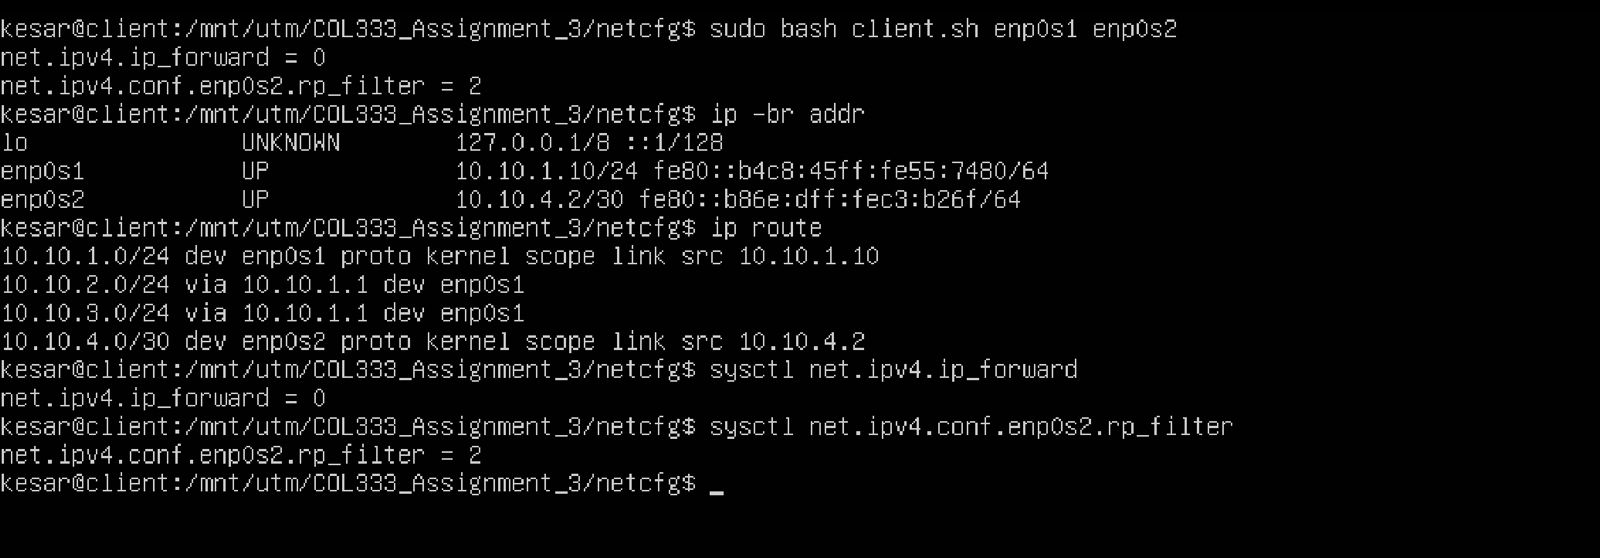
\includegraphics[width=\textwidth]{a1_client_addr_route.jpeg}\\[4pt]
        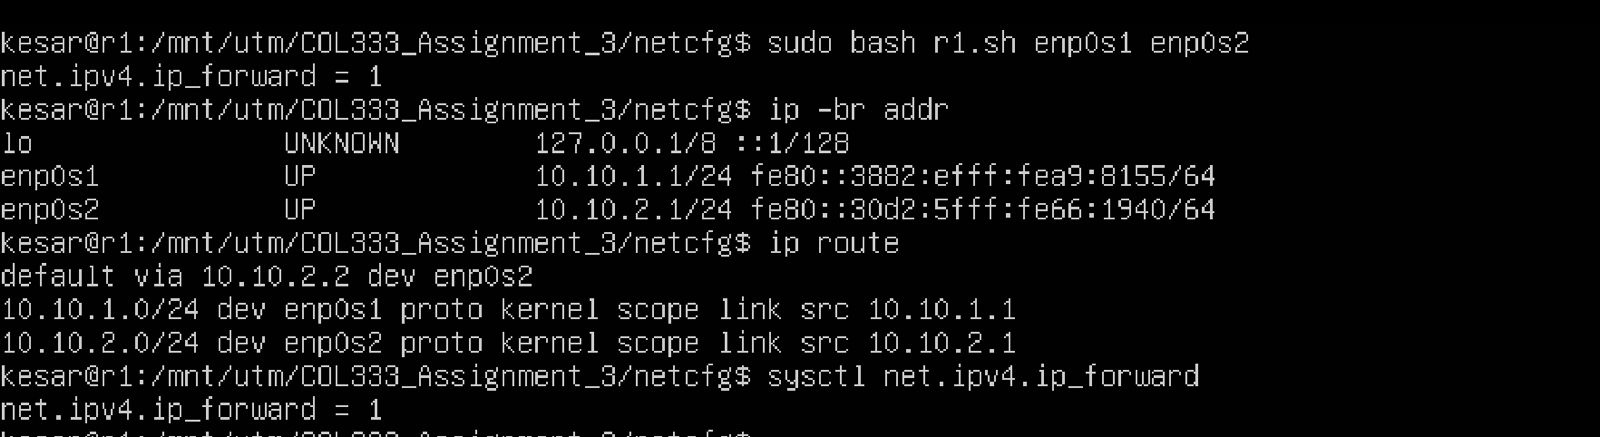
\includegraphics[width=\textwidth]{a1_r1_addr_route.jpeg}\\[4pt]
        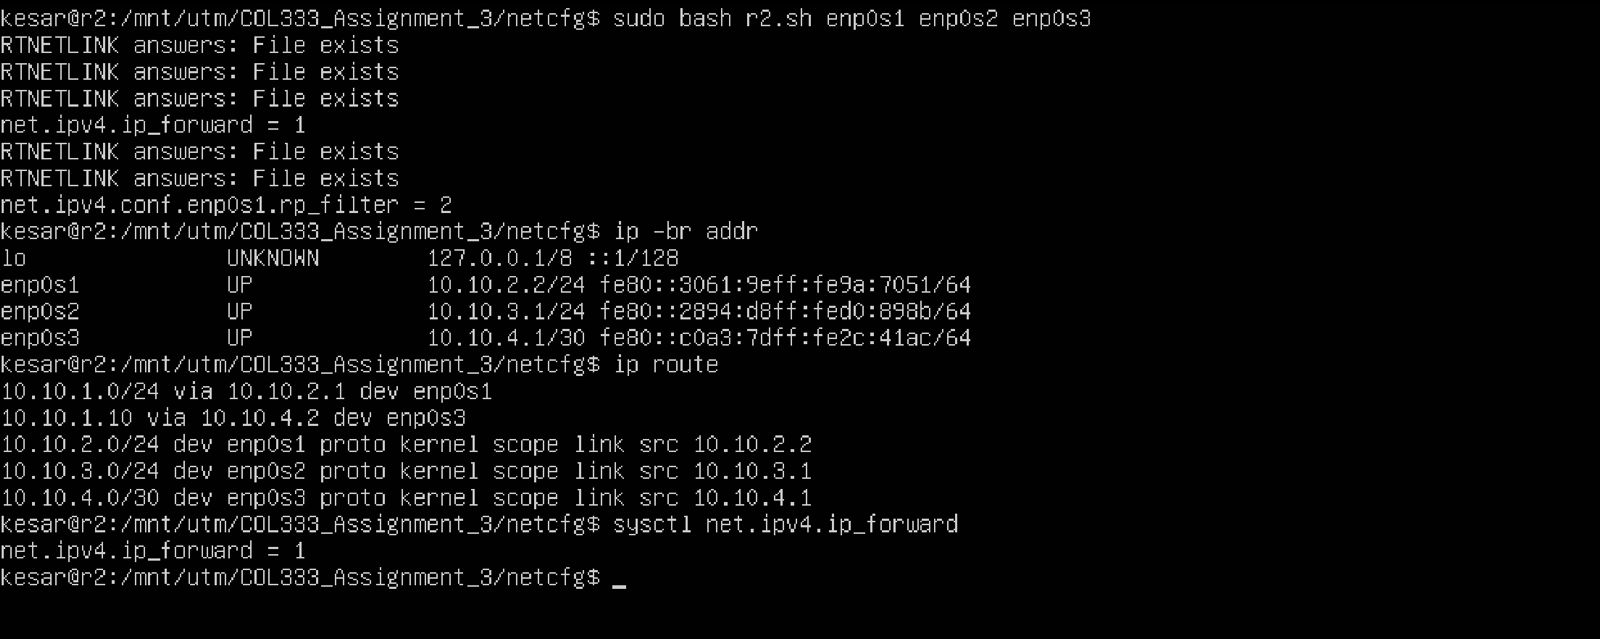
\includegraphics[width=\textwidth]{a1_r2_addr_route.jpeg}\\[4pt]
        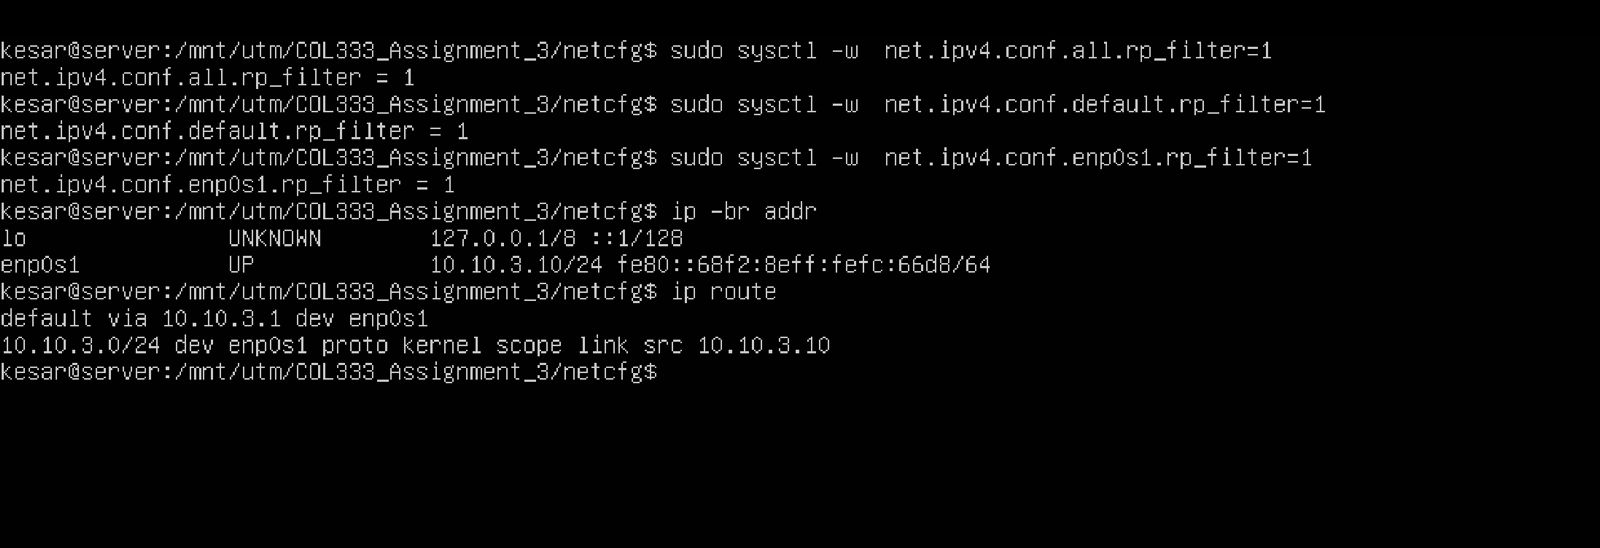
\includegraphics[width=\textwidth]{a1_server_addr_route_again.jpeg}
    \end{minipage}
    \hfill
    \begin{minipage}[t]{0.48\textwidth}
        \centering
        \textbf{Laptop 2}\\[3pt]
        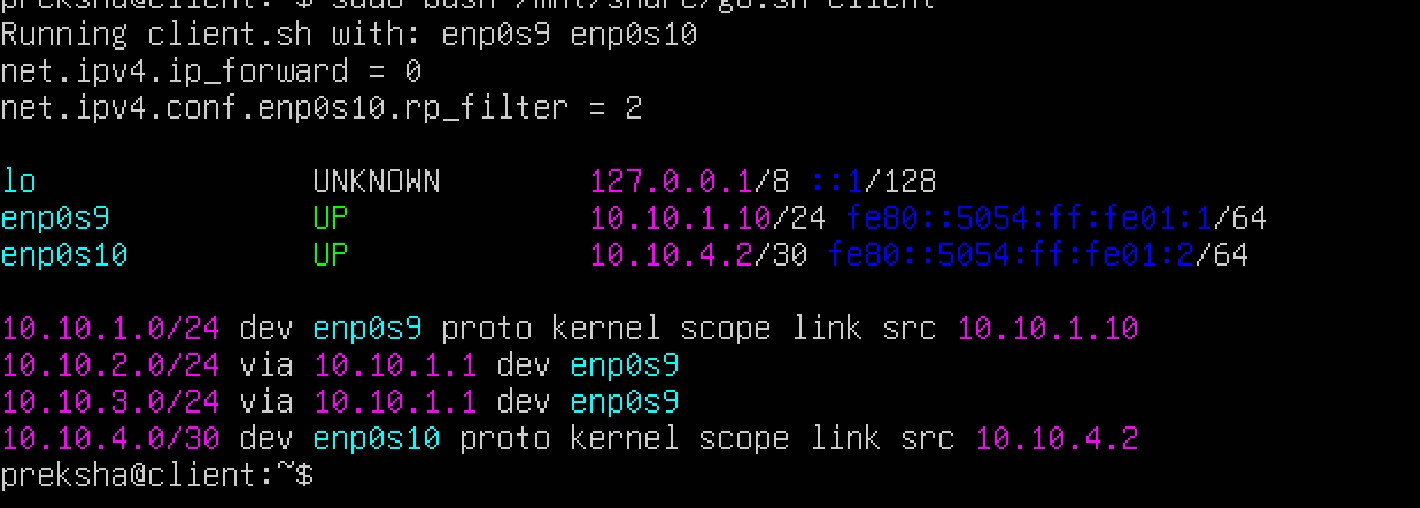
\includegraphics[width=\textwidth]{preksha_r1_client.jpeg}\\[4pt]
        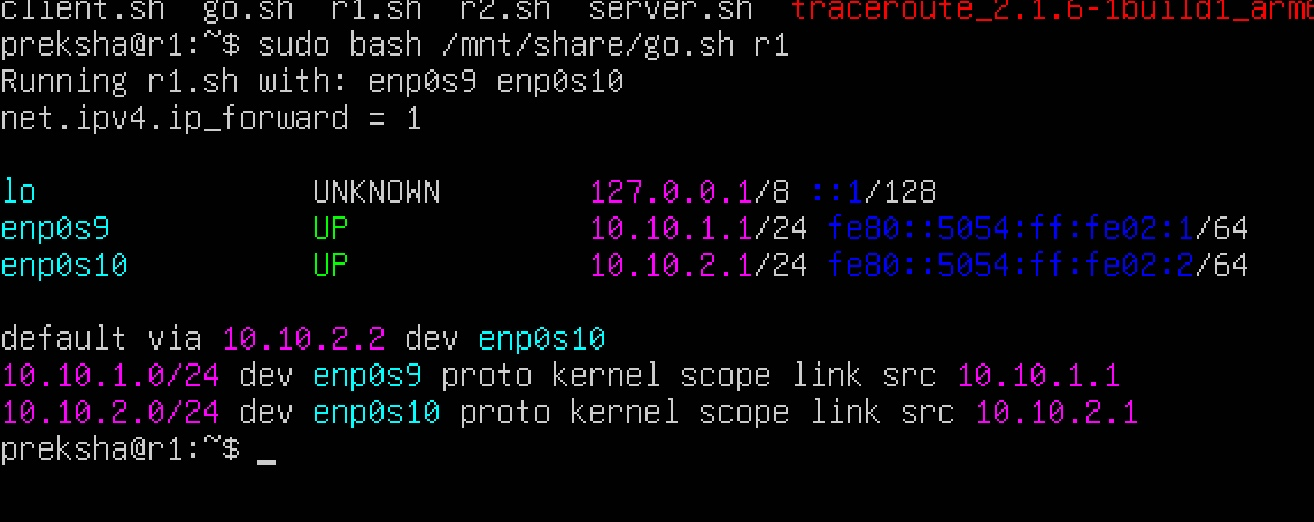
\includegraphics[width=\textwidth]{preksha_r1_r1.jpeg}\\[4pt]
        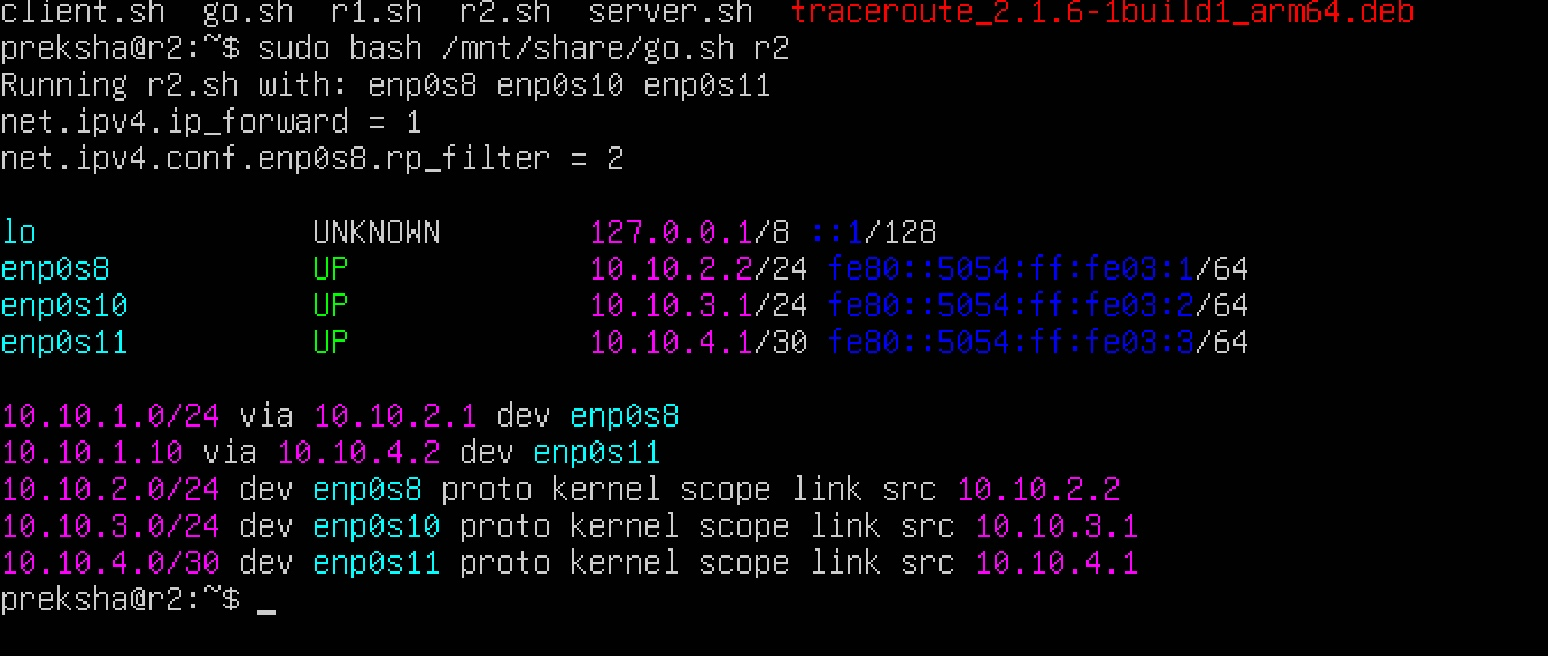
\includegraphics[width=\textwidth]{preksha_r1_r2.jpeg}\\[4pt]
        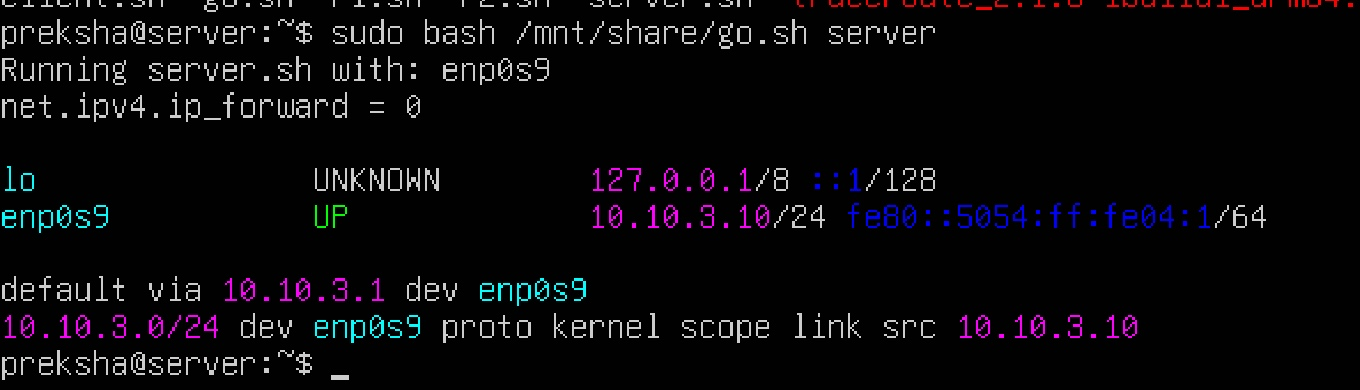
\includegraphics[width=\textwidth]{preksha_r1_server.jpeg}
    \end{minipage}
    \caption{Address assignments and routing-table evidence from both laptop environments.}
    \label{fig:address-route-evidence}
\end{figure}

Connectivity was verified with ping and traceroute. The client-to-server trace follows client $\rightarrow$ r1 $\rightarrow$ r2 $\rightarrow$ server; r2 responds using its Link D address, 10.10.4.1, because the probes reach it over that interface. The server-to-client trace follows server $\rightarrow$ r2 $\rightarrow$ client, using Link D for the final hop. These results confirm the intended asymmetric paths.

% SECTION R2: TRACEROUTE & ASYMMETRIC PATH ANALYSIS
% ==============================================================================

\section{R2: Traceroute and Asymmetric Routing}
\label{sec:r2}

\subsection{Bidirectional Traceroute Results}

We ran {traceroute -n} between the client and server on both laptop environments. Both showed the expected asymmetric paths: three hops from client to server and two hops in the reverse direction.

\begin{figure}[H]
    \centering
    \begin{minipage}[t]{0.48\textwidth}
        \centering
        \textbf{Laptop 1}\\[3pt]
        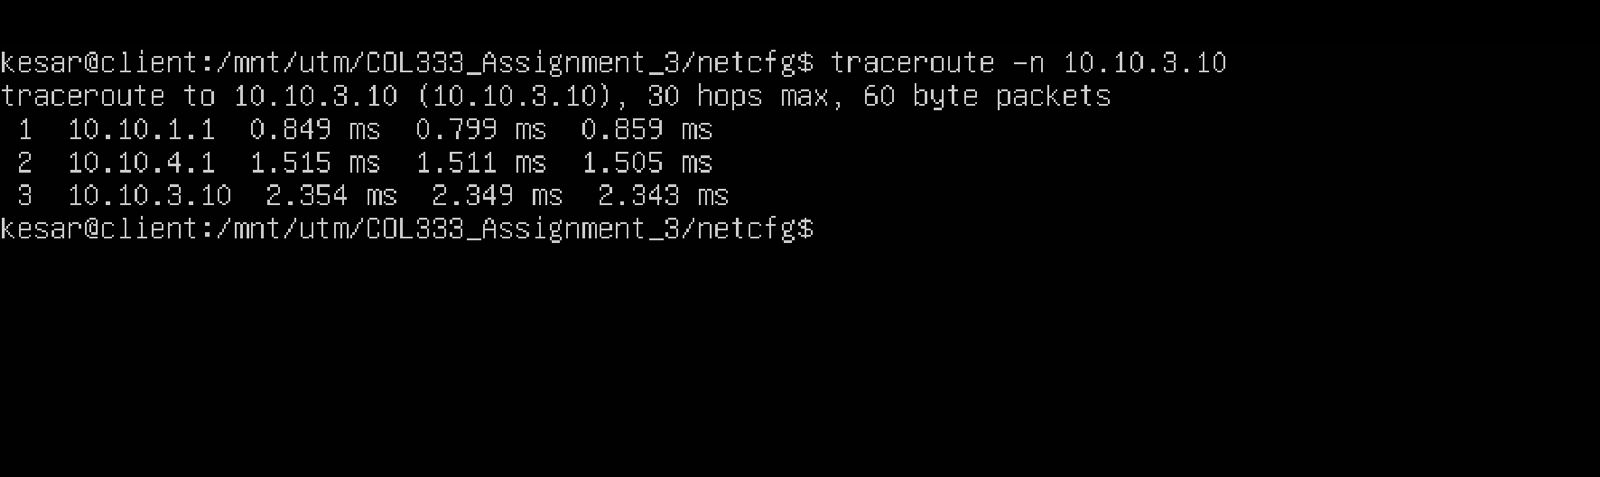
\includegraphics[width=\textwidth]{a3_traceroute_ctos.jpeg}\\
        (a) Client $\rightarrow$ Server (3 hops)\\[5pt]
        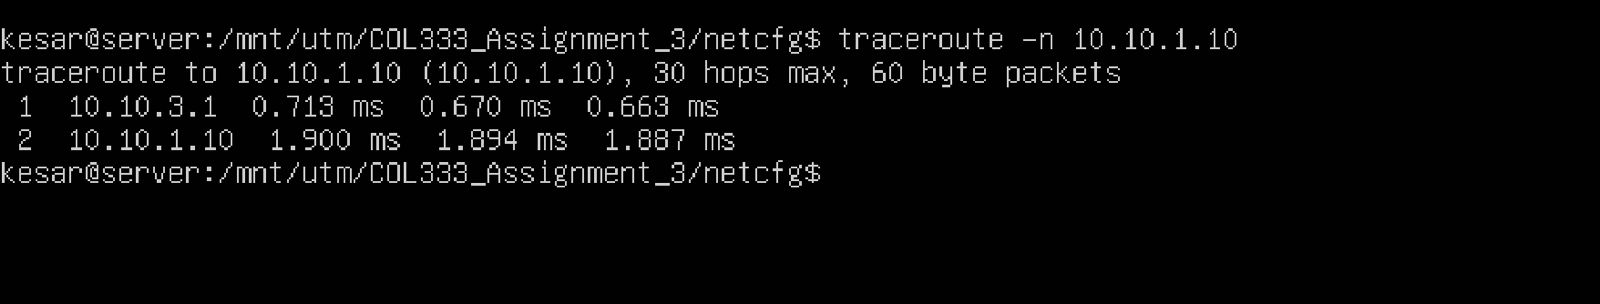
\includegraphics[width=\textwidth]{a3_traceroute_stoc.jpeg}\\
        (b) Server $\rightarrow$ Client (2 hops)
    \end{minipage}
    \hfill
    \begin{minipage}[t]{0.48\textwidth}
        \centering
        \textbf{Laptop 2}\\[3pt]
        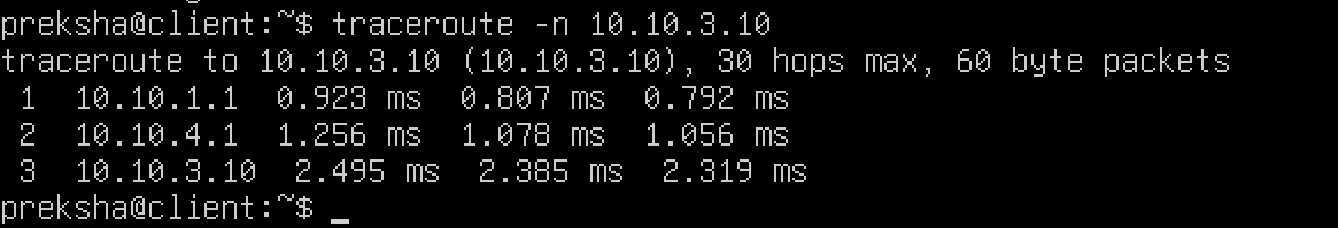
\includegraphics[width=\textwidth]{images_preksha_r1_r5/preksha_r2_traceroute_ctos.jpeg}\\
        (a) Client $\rightarrow$ Server (3 hops)\\[5pt]
        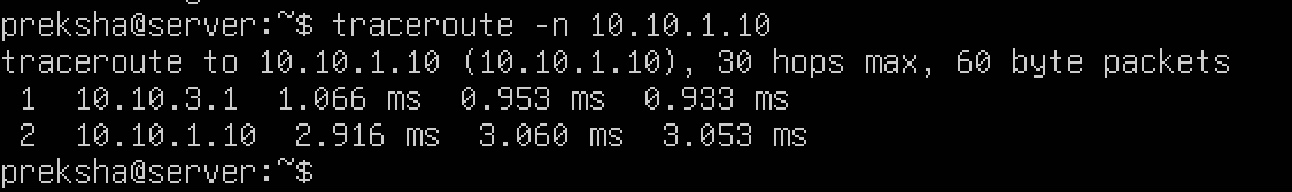
\includegraphics[width=\textwidth]{images_preksha_r1_r5/preksha_r2_traceroute_stoc.jpeg}\\
        (b) Server $\rightarrow$ Client (2 hops)
    \end{minipage}
    \caption{Bidirectional traceroute results from both laptop environments.}
    \label{fig:traceroute_comparison}
\end{figure}

\begin{table}[H]
    \centering
    \renewcommand{\arraystretch}{1.15}
    \begin{tabularx}{\textwidth}{@{} c l l X @{}}
        \toprule
        \textbf{Hop} & \textbf{Client $\rightarrow$ Server} &
        \textbf{Server $\rightarrow$ Client} & \textbf{Explanation} \\
        \midrule
        1 & 10.10.1.1 (r1) & 10.10.3.1 (r2) &
        The first router reached from each endpoint. \\
        2 & 10.10.4.1 (r2) & 10.10.1.10 (client) &
        Forward probes reach r2 over Link D; reverse traffic reaches the client directly over Link D. \\
        3 & 10.10.3.10 (server) & . &
        The forward trace reaches the server after r1 and r2. \\
        \bottomrule
    \end{tabularx}
    \caption{Observed hops in both directions.}
    \label{tab:traceroute_comparison}
\end{table}

\subsection{Explanation of the Asymmetric Paths}

The client routes traffic for the server's subnet, 10.10.3.0/24, through r1. R1 forwards it to r2 using its default route via 10.10.2.2, and r2 delivers it to the server over LAN C. The forward path is therefore:

\[
\text{Client} \rightarrow \text{r1} \rightarrow \text{r2}
\rightarrow \text{Server}.
\]

For return traffic, the server uses its default route via 10.10.3.1 to reach r2. R2 has a specific host route for 10.10.1.10/32 via 10.10.4.2, which takes precedence over its broader route for LAN A via r1. It therefore sends packets directly to the client over Link D, bypassing r1:

\[
\text{Server} \rightarrow \text{r2} \rightarrow \text{Client}.
\]

\subsection{Why r2 Appears as 10.10.4.1}

In the client-to-server trace, r2 appears as 10.10.4.1 rather than 10.10.2.2. Traceroute probes arrive at r2 over LAN B, but r2's route back to the probe source, 10.10.1.10, uses Link D via 10.10.4.2. When r2 generates an ICMP Time Exceeded response, its source address is selected from the outgoing interface, Link D (10.10.4.1). The client therefore reports 10.10.4.1 as the second hop.

\newpage

% ==============================================================================
% SECTION R3: REVERSE-PATH FILTERING ARCHITECTURE
% ==============================================================================

\section{R3: Reverse-Path Filtering}
\label{sec:r3}

\subsection{Modes and Effective Setting}

Linux reverse-path filtering ({rp\_filter}) validates packet source addresses against the routing table:

\begin{itemize}
    \item \textbf{0: Disabled:} No reverse-path validation.
    \item \textbf{1: Strict:} Drops a packet if the best reverse route to its source uses a different interface from the one on which it arrived.
    \item \textbf{2: Loose:} Accepts a packet if its source is reachable through any interface.
\end{itemize}

The effective setting is the maximum of the global and interface-specific values:
\[
\text{effective rp\_filter}
= \max(conf.all.rp\_filter,
       conf.IF.rp\_filter).
\]
All VMs start with strict filtering enabled.

\subsection{Interface Settings and Justification}

\begin{table}[H]
    \centering
    \renewcommand{\arraystretch}{1.15}
    \begin{tabularx}{\textwidth}{@{} l l c X @{}}
        \toprule
        \textbf{Machine} & \textbf{Interface} & \textbf{Mode} &
        \textbf{Reason} \\
        \midrule
        client & LAN A & 1 (Strict) &
        Traffic on the client LAN follows the expected route. \\
        client & Link D & 2 (Loose) &
        Server replies arrive on Link D, although the route back to the server uses LAN A. \\
        r1 & All & 1 (Strict) &
        Forwarding between LAN A and LAN B is compatible with strict filtering. \\
        r2 & LAN B & 2 (Loose) &
        Client packets arrive via r1 on LAN B, but the route back to the client uses Link D. \\
        r2 & LAN C, Link D & 1 (Strict) &
        Strict filtering is retained on the other interfaces. \\
        server & LAN C & 1 (Strict) &
        Server traffic uses LAN C through gateway 10.10.3.1. \\
        \bottomrule
    \end{tabularx}
    \caption{Reverse-path filtering configuration and rationale.}
    \label{tab:rp_filter_table}
\end{table}

Loose filtering is required at two points because the forward and return paths differ:

\begin{itemize}
    \item \textbf{Client, Link D:} Replies from server (10.10.3.10) arrive on Link D, but the client's route to that source uses LAN A via r1. Strict filtering would reject these replies; loose filtering permits them because the source remains reachable.
    
    \item \textbf{r2, LAN B:} Packets from client (10.10.1.10) arrive through r1 on LAN B, while r2's specific host route to the client uses Link D via 10.10.4.2. Strict filtering would reject these packets; loose filtering allows them.
\end{itemize}

R1 and the server retain strict filtering, as their required traffic paths are compatible with it. This preserves the specified filtering policy while allowing the asymmetric routes.

\subsection{Verification Evidence}

We verified IP forwarding and reverse-path filtering on both laptop environments. The screenshots below show the relevant sysctl values and, where available, interface-specific overrides.

\begin{figure}[H]
    \centering
    \begin{minipage}[t]{0.48\textwidth}
        \centering
        \textbf{Laptop 1}\\[4pt]
        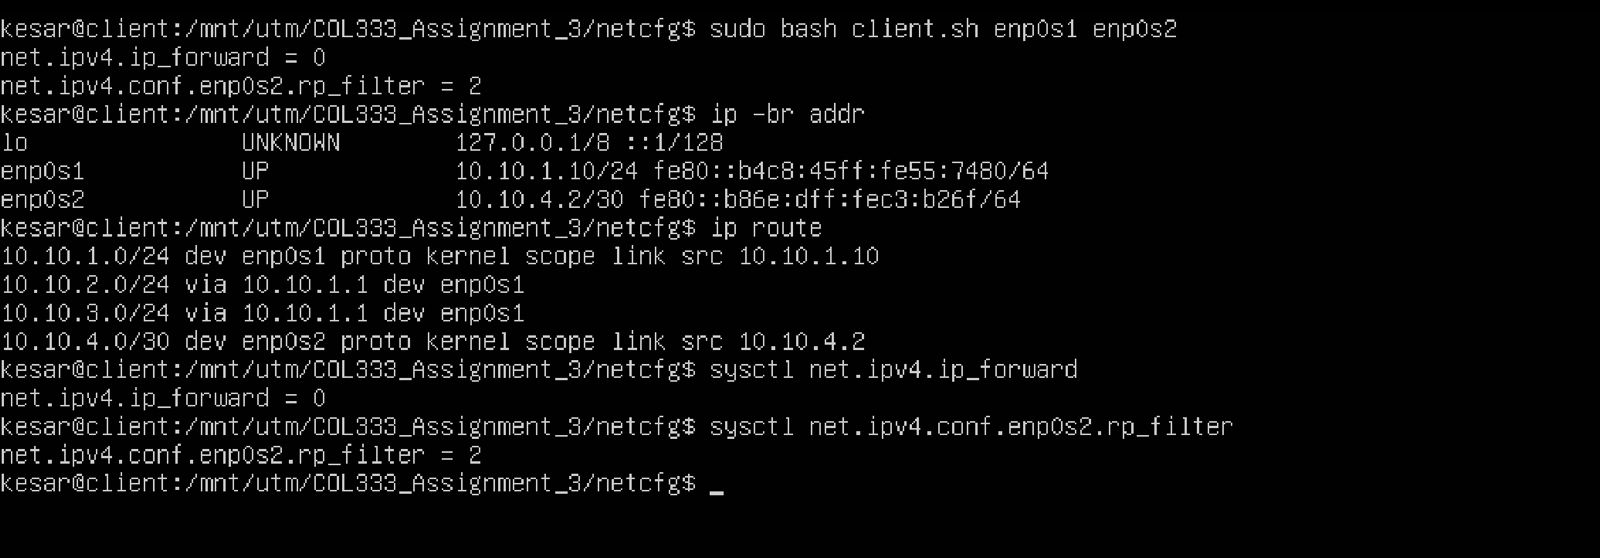
\includegraphics[width=\textwidth]{a1_client_addr_route.jpeg}\\[3pt]
        (a) Client: forwarding disabled; Link D filtering set to loose mode.
    \end{minipage}
    \hfill
    \begin{minipage}[t]{0.48\textwidth}
        \centering
        \textbf{Laptop 2}\\[4pt]
        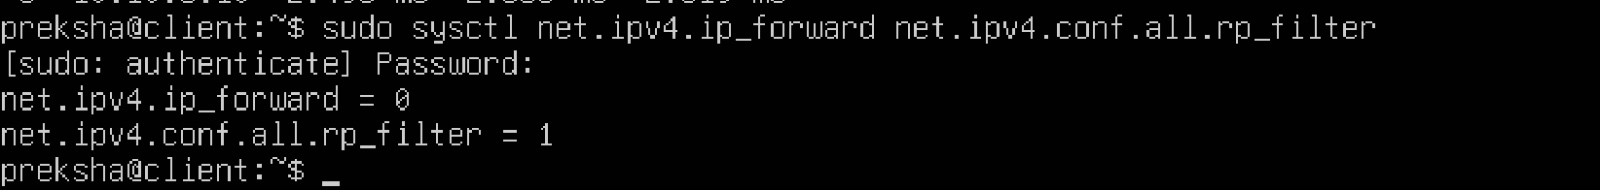
\includegraphics[width=\textwidth]{preksha_r3_client.jpeg}\\[3pt]
        (b) Client: forwarding disabled; global reverse-path filtering set to strict mode.
    \end{minipage}
    
    \label{fig:r3_client_evidence}
\end{figure}

\begin{figure}[H]
    \centering
    \begin{minipage}[t]{0.48\textwidth}
        \centering
        \textbf{Laptop 1}\\[4pt]
        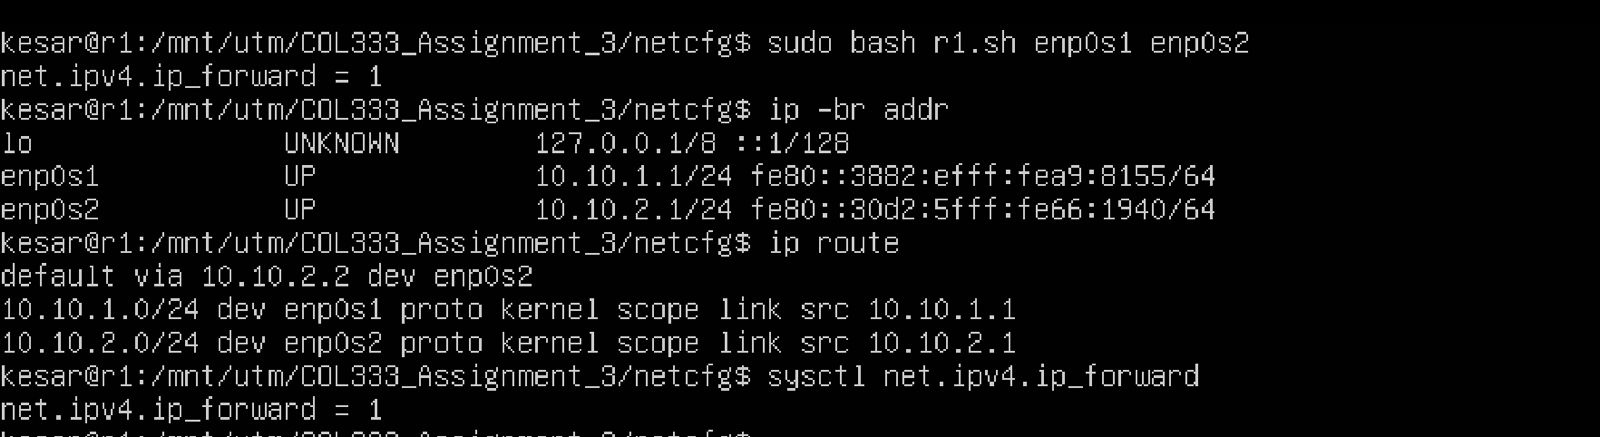
\includegraphics[width=\textwidth]{a1_r1_addr_route.jpeg}\\[3pt]
        (a) r1: forwarding enabled; default route via 10.10.2.2.
    \end{minipage}
    \hfill
    \begin{minipage}[t]{0.48\textwidth}
        \centering
        \textbf{Laptop 2}\\[4pt]
        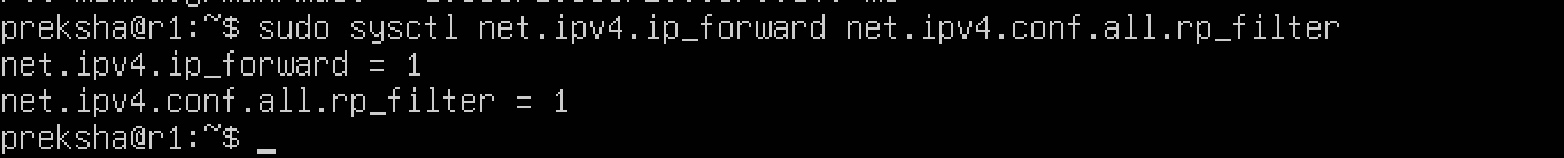
\includegraphics[width=\textwidth]{preksha_r3_r1.jpeg}\\[3pt]
        (b) r1: forwarding enabled; global reverse-path filtering set to strict mode.
    \end{minipage}
    
    \label{fig:r3_r1_evidence}
\end{figure}

\begin{figure}[H]
    \centering
    \begin{minipage}[t]{0.48\textwidth}
        \centering
        \textbf{Laptop 1}\\[4pt]
        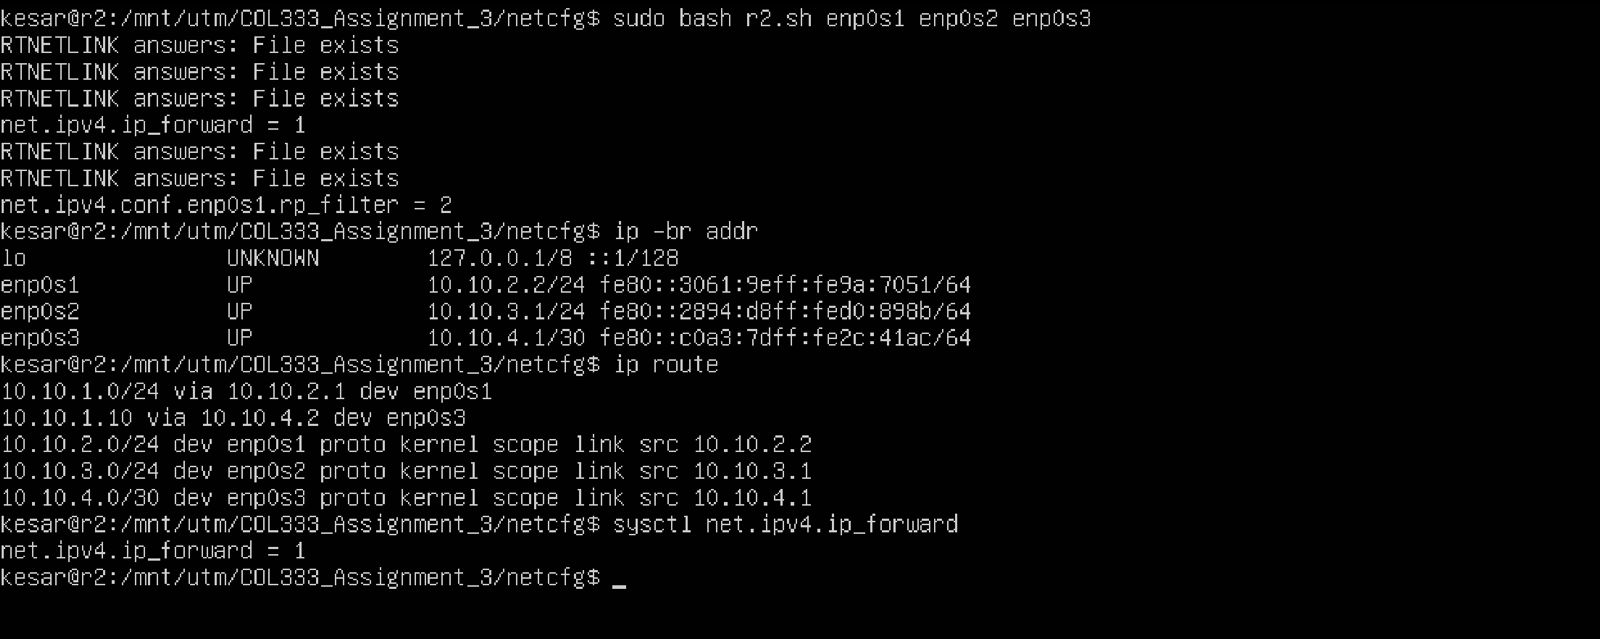
\includegraphics[width=\textwidth]{a1_r2_addr_route.jpeg}\\[3pt]
        (a) r2: forwarding enabled; loose filtering on LAN B.
    \end{minipage}
    \hfill
    \begin{minipage}[t]{0.48\textwidth}
        \centering
        \textbf{Laptop 2}\\[4pt]
        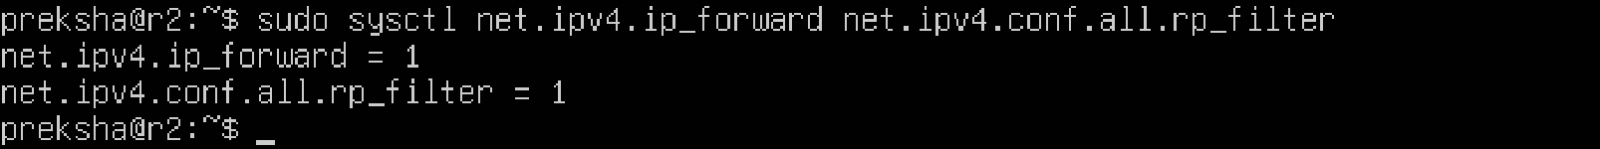
\includegraphics[width=\textwidth]{preksha_r3_r2.jpeg}\\[3pt]
        (b) r2: forwarding enabled; global reverse-path filtering set to strict mode.
    \end{minipage}
    
    \label{fig:r3_r2_evidence}
\end{figure}

\begin{figure}[H]
    \centering
    \begin{minipage}[t]{0.48\textwidth}
        \centering
        \textbf{Laptop 1}\\[4pt]
        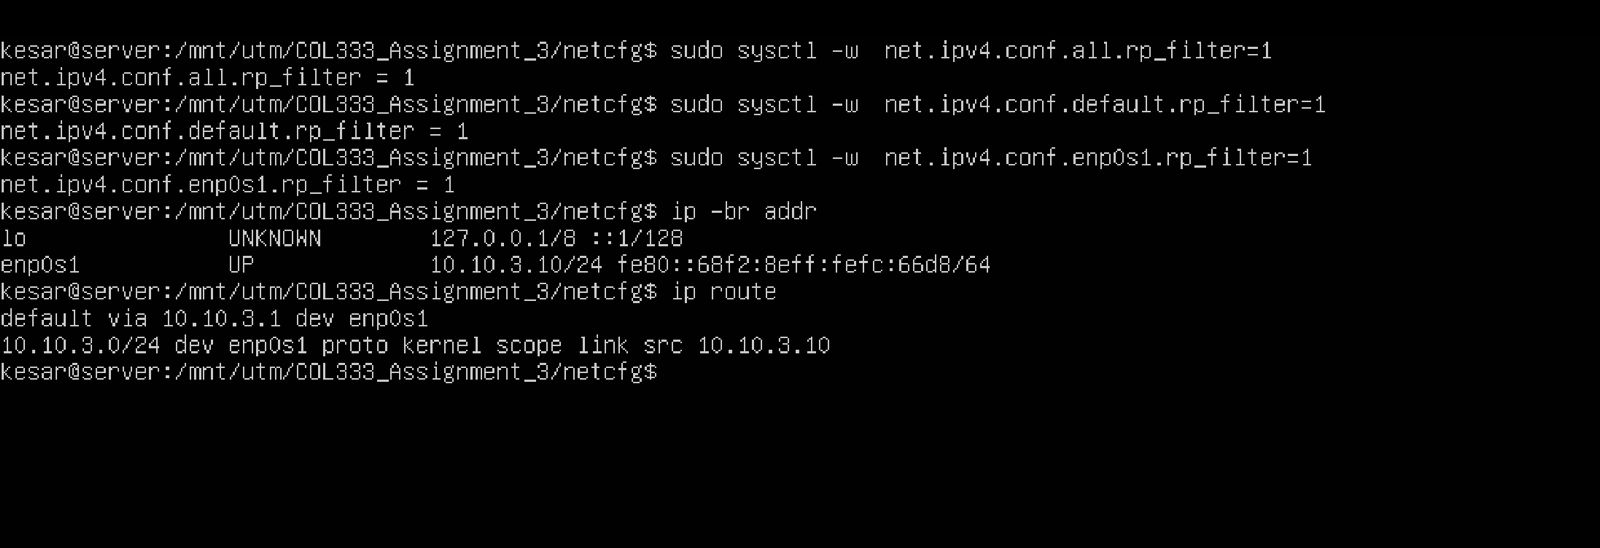
\includegraphics[width=\textwidth]{a1_server_addr_route_again.jpeg}\\[3pt]
        (a) Server: forwarding disabled; strict filtering configured on the interface.
    \end{minipage}
    \hfill
    \begin{minipage}[t]{0.48\textwidth}
        \centering
        \textbf{Laptop 2}\\[4pt]
        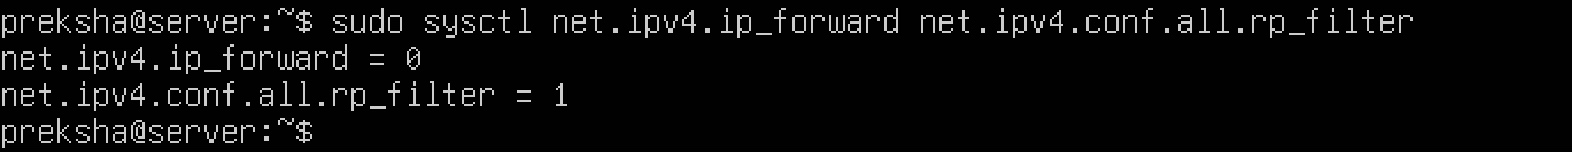
\includegraphics[width=\textwidth]{preksha_r3_server.jpeg}\\[3pt]
        (b) Server: forwarding disabled; global reverse-path filtering set to strict mode.
    \end{minipage}
    
    \label{fig:r3_server_evidence}
\end{figure}

The screenshots confirm the required forwarding settings: forwarding is disabled on the client and server and enabled on r1 and r2. They also show the global strict-filter setting and the loose interface-specific overrides where captured. Interface-specific values not visible in a screenshot should be verified separately before claiming they were confirmed on both laptops.

\newpage

% ==============================================================================
% SECTION R4: CUSTOM HTTP CLIENT WITH STANDARD HTTP SERVER
% ==============================================================================

\section{R4: Custom TCP Client with a Standard HTTP Server}
\label{sec:r4}

\subsection{Setup}

We tested the custom HTTP client against Python's standard HTTP server, running on the server VM at 10.10.3.10:8000. The server provided two files:

\begin{itemize}
    \item \textbf{output.html}: 22 bytes.
    \item \textbf{large\_file.bin}: 150 KB (153,600 bytes), generated using {/dev/urandom}.
\end{itemize}

For raw TCP socket interoperability, GRO was disabled on the relevant interface and kernel-generated TCP RST packets were filtered using iptables.

\subsection{Download and Integrity Verification}

We downloaded both objects using the custom client and {curl}. The downloads completed with exit code 0, and the MD5 hashes matched between the original files and the downloaded copies.

\begin{table}[H]
    \centering
    \renewcommand{\arraystretch}{1.2}
    \begin{tabularx}{\textwidth}{@{} l r l X @{}}
        \toprule
        \textbf{File} & \textbf{Size} & \textbf{Exit Code} &
        \textbf{MD5 Checksum} \\
        \midrule
        output.html & 22 B & 0 &
        {ad92f9a5ee8aee56f44ac52d8096afe0} \\
        large\_file.bin & 153,600 B & 0 &
        {2779b51746afc991dd6886b1fa1ffaed} \\
        \bottomrule
    \end{tabularx}
    \caption{Downloaded file sizes, exit codes, and verified MD5 checksums.}
    \label{tab:r4_md5_table}
\end{table}

\subsection{Experimental Evidence}

Figures~\ref{fig:r4_client_evidence} and~\ref{fig:r4_server_evidence} show the download results and server logs from both laptop environments.


\begin{figure}[H]
    \centering
    \begin{minipage}[t]{0.48\textwidth}
        \centering
        \textbf{Laptop 1}\\[3pt]
        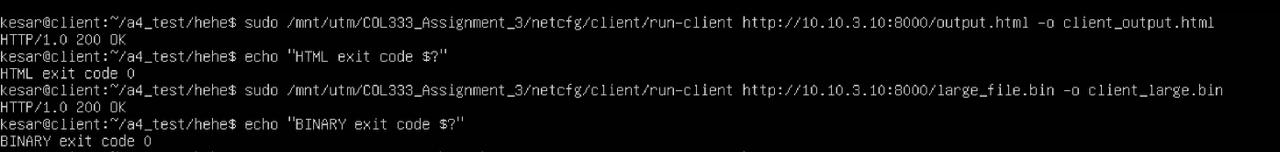
\includegraphics[width=\textwidth]{r4_p1_client.jpeg}\\
        (a) Client download results\\[5pt]
        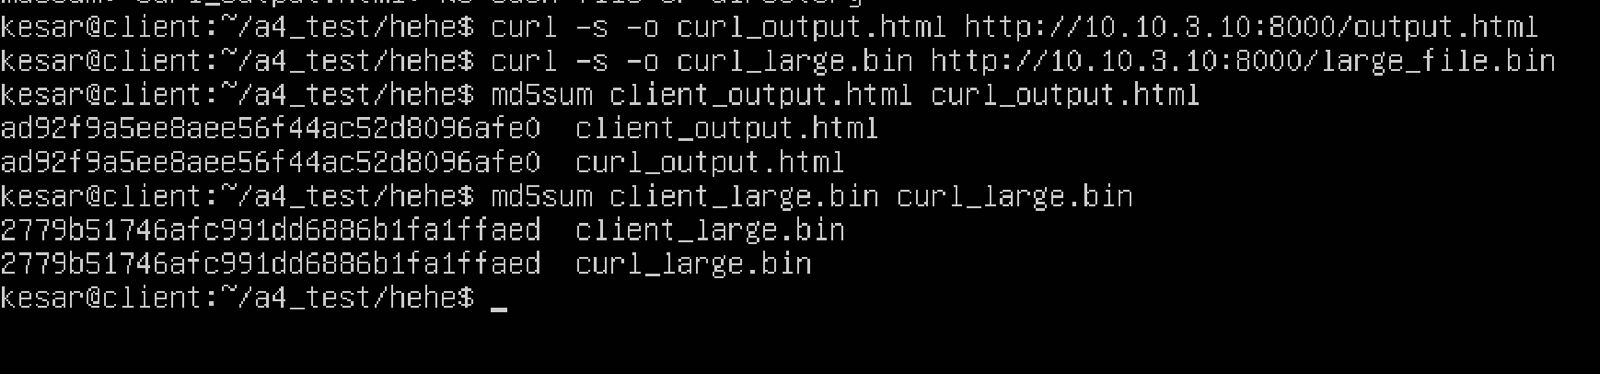
\includegraphics[width=\textwidth]{r4_p2_client.jpeg}\\
        (b) Curl and MD5 comparison
    \end{minipage}
    \hfill
    \begin{minipage}[t]{0.48\textwidth}
        \centering
        \textbf{Laptop 2}\\[3pt]
        \includegraphics[width=\textwidth]{sub1.png}\\
        (a) Client download results\\[5pt]
        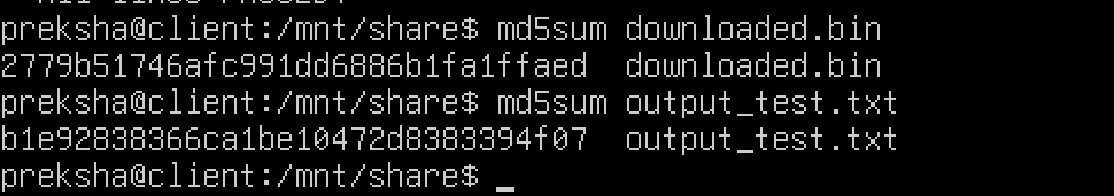
\includegraphics[width=\textwidth]{preksha_r4_md5.jpeg}\\
        (b) MD5 verification
    \end{minipage}
    \label{fig:r4_client_evidence}
\end{figure}

\begin{figure}[H]
    \centering
    \begin{minipage}[t]{0.48\textwidth}
        \centering
        \textbf{Laptop 1}\\[3pt]
        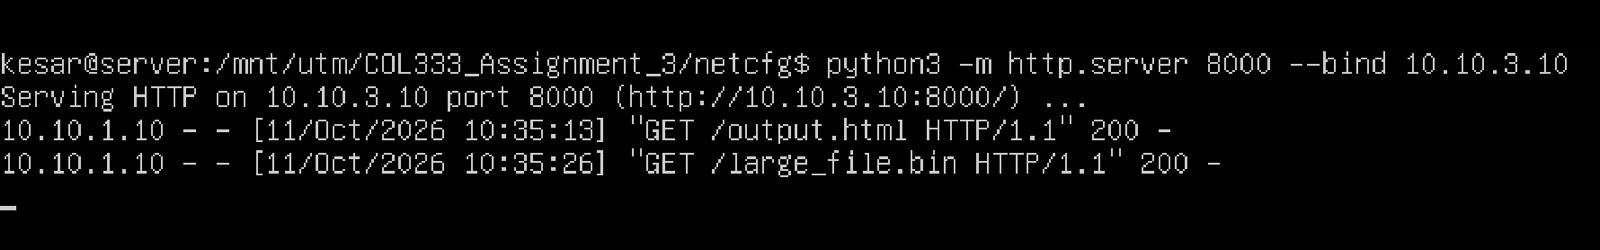
\includegraphics[width=\textwidth]{r4_p1_server.jpeg}
    \end{minipage}
    \hfill
    \begin{minipage}[t]{0.48\textwidth}
        \centering
        \textbf{Laptop 2}\\[3pt]
        % Replace with the actual server-log screenshot from Laptop 2,
        % if available.
        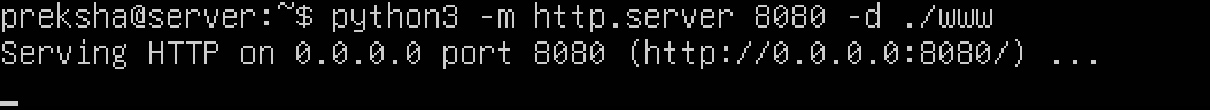
\includegraphics[width=\textwidth]{preksha_r4_server.jpeg}
    \end{minipage}
    \label{fig:r4_server_evidence}
\end{figure}

The matching MD5 checksums confirm that the downloaded files are byte-for-byte identical to the originals. The server logs provide additional evidence that the requests reached the server and were handled.

\newpage

% ==============================================================================
% SECTION R5: CLIENT-SERVER INTEROPERATION
% ==============================================================================
\section{R5: Client--Server Interoperation}
\label{sec:r5}

\subsection{Setup}

We tested the custom HTTP server on 10.10.3.10:8080 using three clients: {curl}, {wget}, and our custom HTTP client. Each downloaded {large\_file.bin} (153,600 bytes) from the server.

\subsection{Results and Integrity Verification}

All three downloads completed successfully. Their MD5 checksums matched the original file, confirming byte-for-byte integrity.

\begin{table}[H]
    \centering
    \renewcommand{\arraystretch}{1.15}
    \setlength{\tabcolsep}{8pt}
    \begin{tabularx}{0.95\textwidth}{@{} l l X @{}}
        \toprule
        \textbf{Client} & \textbf{Output file} & \textbf{MD5 checksum} \\
        \midrule
        Server original & {large\_file.bin} &
        {\small{2779b51746afc991dd6886b1fa1ffaed}} \\
        {curl} & {curl\_r5.bin} &
        {\small{2779b51746afc991dd6886b1fa1ffaed}} \\
        {wget} & {wget\_r5.bin} &
        {\small{2779b51746afc991dd6886b1fa1ffaed}} \\
        Custom client & {client\_r5.bin} &
        {\small{2779b51746afc991dd6886b1fa1ffaed}} \\
        \bottomrule
    \end{tabularx}
    \caption{MD5 checksums of the original file and all downloaded copies.}
    \label{tab:r5_summary}
\end{table}


\subsection{Experimental Evidence}

The following screenshots show the client-side downloads and checksum comparisons, together with the server-side execution, on both laptop environments.

\begin{figure}[H]
    \centering
    \begin{minipage}[t]{0.48\textwidth}
        \centering
        \textbf{Laptop 1}\\[3pt]
        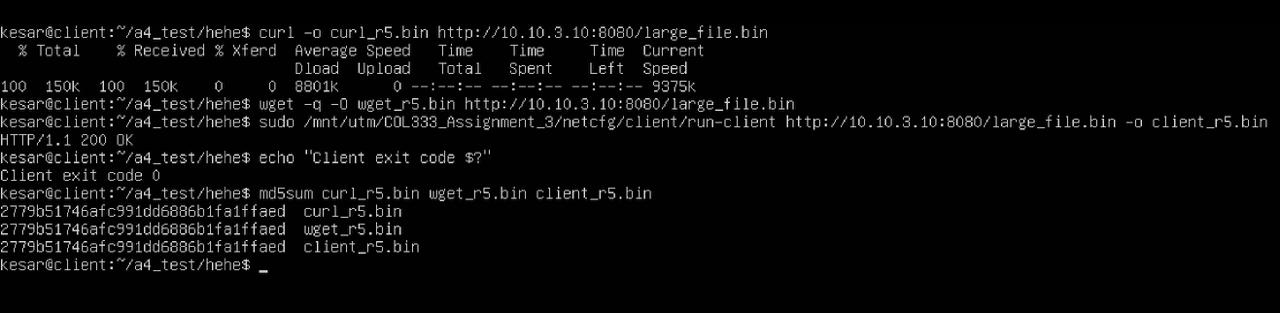
\includegraphics[width=\textwidth]{r5_client.jpeg}\\
        (a) Client downloads and MD5 results\\[5pt]
        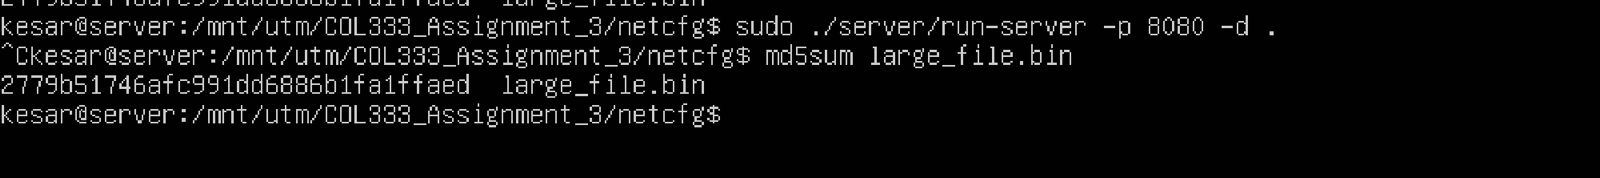
\includegraphics[width=\textwidth]{r5_server.jpeg}\\
        (b) Custom server and original file checksum
    \end{minipage}
    \hfill
    \begin{minipage}[t]{0.48\textwidth}
        \centering
        \textbf{Laptop 2}\\[3pt]
        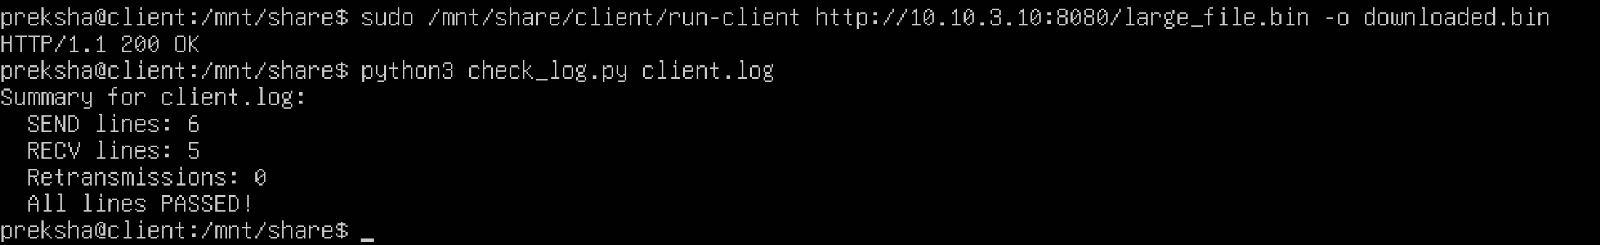
\includegraphics[width=\textwidth]{preksha_r5_client.jpeg}\\
        (a) Custom client download\\[5pt]
        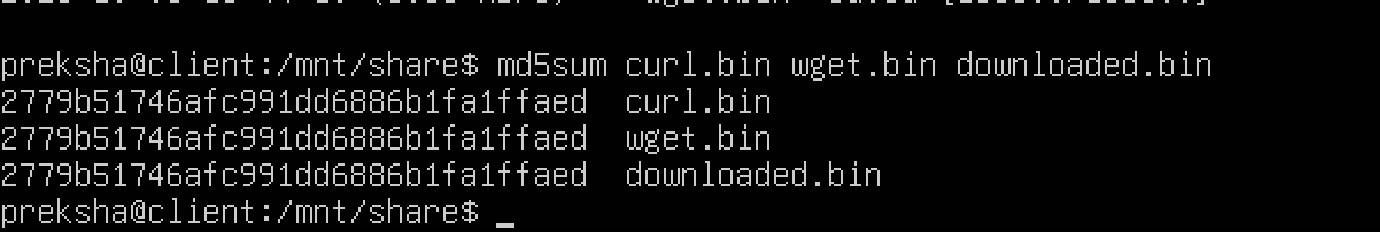
\includegraphics[width=\textwidth]{preksha_r5_md5.jpeg}\\
        (b) Client checksum comparison
    \end{minipage}
    \caption{Interoperation and integrity verification in both laptop environments.}
    \label{fig:r5_evidence}
\end{figure}

Matching checksums demonstrate that the downloaded contents are identical to the original file. The results verify interoperation between standard HTTP clients and the custom server, as well as successful use of the custom client, provided each recorded transfer completed successfully.

\newpage

% ==============================================================================
% SECTION R6: PACKET CAPTURE & TCP DESIGN ARCHITECTURE
% ==============================================================================

\section{R6: Packet Capture and TCP Implementation}
\label{sec:r6}

\subsection{TCP Connection Capture}

We captured the custom client's download of {output.html} using {tcpdump -nn}. The 11 packets show the TCP handshake, HTTP request and response, and orderly connection teardown.

\begin{figure}[H]
    \centering
    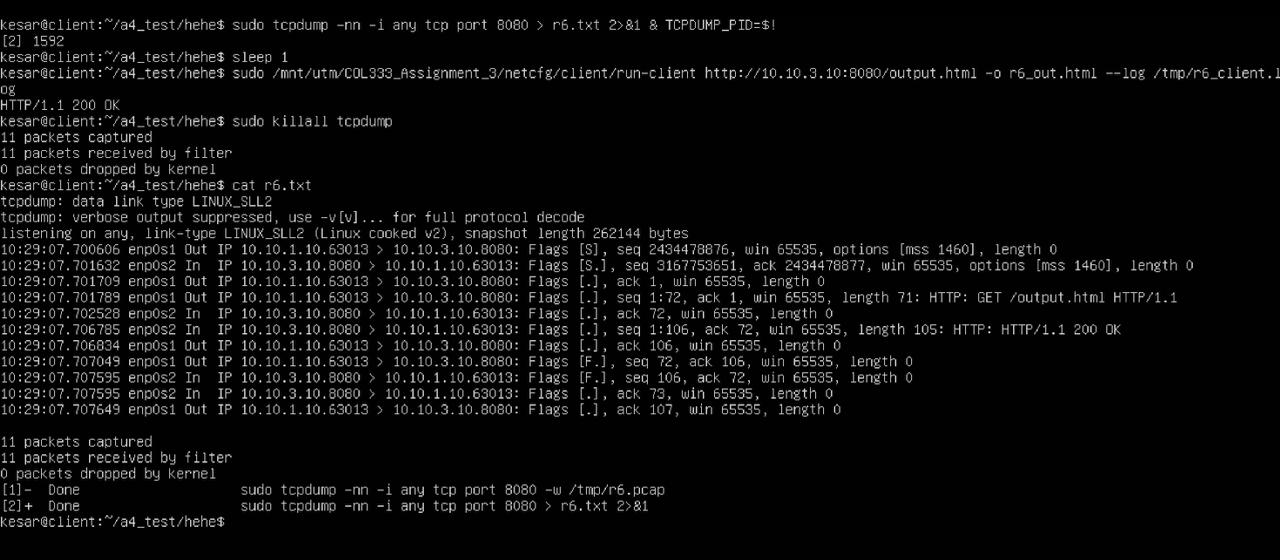
\includegraphics[width=0.95\textwidth]{r6_client.jpeg}
    \caption{Packet capture of the custom client's HTTP request to the custom server.}
    \label{fig:tcpdump_capture}
\end{figure}

\begin{table}[H]
    \centering
    \renewcommand{\arraystretch}{1.15}
    \begin{tabularx}{\textwidth}{@{} c l X @{}}
        \toprule
        \textbf{Packets} & \textbf{Direction and flags} & \textbf{Purpose} \\
        \midrule
        1-3 & Client $\leftrightarrow$ Server; SYN, SYN-ACK, ACK &
        Complete the three-way handshake. The SYN-ACK arrives on the client's Link D interface. \\
        4-5 & Client $\rightarrow$ Server; PSH-ACK, ACK &
        Send the HTTP GET request and acknowledge its receipt. \\
        6-7 & Server $\rightarrow$ Client; PSH-ACK, ACK &
        Return the HTTP response (105 bytes, including headers and the 22-byte body) and acknowledge it. \\
        8-11 & Client $\leftrightarrow$ Server; FIN-ACK, ACK &
        Close the connection cleanly using FIN and ACK packets. \\
        \bottomrule
    \end{tabularx}
    \caption{Summary of the 11-packet TCP connection.}
    \label{tab:r6_packets}
\end{table}

The client sends its SYN over LAN A, while the SYN-ACK returns over Link D. This is consistent with the configured asymmetric routing. The exchange then completes the HTTP transfer and closes the connection without a reset in the captured sequence.

\subsection{Retransmission and Timer Management}

The TCP engine tracks unacknowledged segments in an in-flight queue and retransmits them when their retransmission timeout (RTO) expires. RTT samples from eligible, non-retransmitted segments are used to update the smoothed RTT and RTT variance according to RFC 6298 and Karn's algorithm:

\[
\fbox{\(
\begin{aligned}
\mathrm{RTTVAR} &\leftarrow 0.75\,\mathrm{RTTVAR}
+ 0.25\,|\mathrm{SRTT}-\mathrm{Sample}|\\
\mathrm{SRTT} &\leftarrow 0.875\,\mathrm{SRTT}
+ 0.125\,\mathrm{Sample}\\
\mathrm{RTO} &\leftarrow
\min(1.0,\max(0.1,\mathrm{SRTT}+4\,\mathrm{RTTVAR}))\,\mathrm{s}
\end{aligned}
\)}
\]

The implementation caps the RTO at 1.0 s. On timeout, the oldest unacknowledged segment is retransmitted and the timeout is backed off exponentially. Handshake and teardown timers separately enforce the required SYN and FIN retry deadlines.

\subsection{Out-of-Order Buffering and Reassembly}

The receive path maintains the next expected sequence number, \texttt{rcv\_nxt}. Segments arriving ahead of this position are buffered by sequence number if they fall within the receive window. When missing data arrives, contiguous buffered segments are drained into the receive stream and \texttt{rcv\_nxt} advances. Duplicate or overlapping data is trimmed as needed, and cumulative ACKs report the next expected sequence number.

Sequence comparisons account for 32-bit wraparound using modular arithmetic. These mechanisms preserve data order when segments arrive out of order.

\subsection{TCP Reno Congestion Control}

The sender implements TCP Reno using the congestion window (\texttt{cwnd}) and slow-start threshold (\texttt{ssthresh}):

\begin{itemize}
    \item \textbf{Slow start:} While \texttt{cwnd} is below \texttt{ssthresh}, it grows by up to one MSS per newly acknowledged segment, producing approximately exponential growth per RTT.
    
    \item \textbf{Congestion avoidance:} Once \texttt{cwnd} reaches \texttt{ssthresh}, additive increase grows the window by approximately one MSS per RTT:
    \[
\fbox{\(
\displaystyle
\mathrm{cwnd} \leftarrow \mathrm{cwnd}
+ \frac{\mathrm{MSS}^{2}}{\mathrm{cwnd}}
\)}
\]
    
    \item \textbf{Fast retransmit and recovery:} On the third duplicate ACK, the sender retransmits the oldest unacknowledged segment and reduces its sending rate by updating \texttt{ssthresh} and \texttt{cwnd}. Additional duplicate ACKs inflate \texttt{cwnd}; a new cumulative ACK ends recovery.
    
    \item \textbf{Timeout:} On RTO expiry, the sender reduces \texttt{ssthresh}, resets \texttt{cwnd} to one MSS, and returns to slow start.
\end{itemize}

The packet capture verifies the normal connection lifecycle. Retransmission, out-of-order recovery, and congestion-control responses are implementation mechanisms and require suitable loss or reordering tests to demonstrate their behavior experimentally.

\end{document}
